\documentclass[10pt,a4paper]{article}
\usepackage[latin1]{inputenc}
\usepackage{amsmath}
\usepackage{amsfonts}
\usepackage{amssymb}
\usepackage[]{theorem}
\usepackage[hidelinks]{hyperref}

\usepackage{graphicx}



\setlength{\topmargin}{-.5in}
\setlength{\textheight}{9in}
\setlength{\oddsidemargin}{.125in}
\setlength{\textwidth}{6.25in}



\newcommand {\subsubsubsection} [1] {\vskip 0.5em {\bf \em #1}}

%\newcommand {\comm} [1] {}
\newcommand {\comm} [1]
{
\par
\setlength{\leftskip}{-0.8in}
\begin{tabular} {p{0.1cm} | p{\textwidth}}
  {\bf ?} & {#1}
\end{tabular}
\par
\setlength{\leftskip}{0in}
}


\newcommand {\cond} {, & \textrm{if }}
\newcommand {\otherwise} {, & \textrm{else}}

\newcommand {\Forall} {\forall \ }
\newcommand {\eqdef} {\triangleq}
\newcommand {\equivalent} {\Leftrightarrow}
\renewcommand {\implies} {\Rightarrow}
\renewcommand {\impliedby} {\Leftarrow}
\renewcommand {\And}  {\ \& \ }
\newcommand {\Or}  {\ \vee \ }
\newcommand {\QED} {$\square$ \ \par }
\newcommand {\proofword}  {{\par \sf Proof:\ }}
\newcommand {\proof} [1] {\proofword #1 \QED \par}
\newcommand {\definition} [2] {\bigskip {\bf Definition} {\rm \sc #1} \par #2 \QED \bigskip}
\newcommand {\example} [2] {\bigskip {\bf Example.} {#1} \par #2 \QED}
\newcommand {\theorem} [2] {\bigskip {\bf Theorem} {\rm \sc #1} \par #2 \QED \bigskip}
\newcommand {\ve} {\mathbf}
\newcommand {\vecc} {\boldsymbol}
\newcommand {\Questions} {\vspace{5mm} {\bf Unresolved Questions:}}
\newcommand {\assert} {\square \ }

\renewcommand {\P} {\mathrm P}
\newcommand {\E} {\mathrm E \ }
\newcommand {\var} {\mathrm {var} \ }
\newcommand {\cov} {\mathrm {cov} }
\newcommand {\cor} {\mathrm {cor} }
\newcommand {\N} {\mathbb N}
\newcommand {\Z} {\mathrm Z}
\newcommand {\R} {\mathbb R}
\newcommand {\C} {\mathbb C}
\newcommand {\I} {\mathbb I}
\newcommand {\supp} {\mathrm {Supp}}
\newcommand {\mat} {\mathrm}
\newcommand {\trc} {\mathrm {tr} \ }
\newcommand {\VC} {\mathrm {VC} }
\newcommand {\const} {\mathrm {const} }
\newcommand {\sgn} {\mathrm {sgn} }
\newcommand {\dom} {\mathrm {dom} }
\newcommand {\range} {\mathrm {range} }
\newcommand {\Arg} {\mathrm {Arg} \ }

\newcommand {\LCA} {\mathrm {LCA} }  % least common ancestor (in a tree)

\newcommand {\nul} {\mathrm {null}}
\newcommand {\Dt} {\Delta t}
\newcommand {\PC} {\mathrm {PC} }
\newcommand {\MDS} {\mathrm {MDS} }
\newcommand {\CC} {\mathrm {CC} }

\newcommand {\re} {\mathrm {re}}
\newcommand {\cl} {\mathrm {cl}}
\newcommand {\intr} {\mathrm {int}}

\newcommand {\<} {\langle}
\renewcommand {\>} {\rangle}

\newcommand {\dotve} [1] {\dot {\ve #1}}

\newcommand {\la} [1] {\lambda (#1) \ }

\newcommand {\lhs} {\mathrm {lhs}}
\newcommand {\rhs} {\mathrm {rhs}}

\providecommand{\keywords}[1]
{
  \small
  \textbf{\textit{Keywords---}} #1
}

\makeatletter
\DeclareRobustCommand{\cev}[1]{%
  {\mathpalette\do@cev{#1}}%
}
\newcommand{\do@cev}[2]{%
  \vbox{\offinterlineskip
    \sbox\z@{$\m@th#1 x$}%
    \ialign{##\cr
      \hidewidth\reflectbox{$\m@th#1\vec{}\mkern4mu$}\hidewidth\cr
      \noalign{\kern-\ht\z@}
      $\m@th#1#2$\cr
    }%
  }%
}
\makeatother




\title{Classical Multidimensional Scaling for Genome and Protein Comparisons}
\author{Vyacheslav Brover}


\begin{document}
\maketitle

\tableofcontents

\large


\section{Introduction}

Multidimensional scaling (MDS) is one of the basic explorative methods of multivariate data analysis, together with principal component analysis (PCA) and clustering.
MDS is similar to PCA in that a set of new numerical attributes is constructed on which the data points, or objects, are projected,
but is different in that the input for MDS is an object-object table of pairwise distances or similarities between objects,
whereas the input for PCA is an object-attribute table.

However MDS is not as popular in bioinformatics, as PCA, though multiple genome and protein comparisons are abundant,
because the MDS requires that the object-object similarity matrix should be approximately positive semidefinite.

The MDS method uses a double-centered symmetric matrix as input, and constructs centered and non-correlated numerical attributes $y_1, y_2, y_3, \dots, y_q$ as output,
like in PCA, such that $y_1$ has the largest variance, $y_2$ is orthogonal to y1 and has the largest variance, and so on.
If objects make up large clusters located distantly from each other, then the MDS plot will clearly show them.
Therefore, MDS is usually followed by a clustering in the space of the MDS attributes.

If the object-object table of pairwise distances can be represented by a tree, then this is the best representation of the objects,
but only if the tree is constructed by a maximum likelihood estimation (MLE) method.
However, building an MLE tree is an NP-hard problem.
The MDS plot with clusters is better than a tree in an explorative analysis, because it is faster and easier to use.
It also turns out that MDS can reveal some properties of the MLE tree.




\section{Methods}

The dataflow is shown in Fig. {Dataflow}.

\subsection {Matrix of double-centered generalized similarities}

\subsubsection {Generalized distances and similarities}

Let~$\R$ be the set of real numbers and $\I$ be the set of imaginary numbers.

Let a matrix $X_{raw} \in \{\R^n,\I^n\}^p$ be an object-attribute table, the~$n$ rows of which represent objects and the~$p$ columns of which represent numerical attributes.
Each attribute is either in real or imaginary numbers.
This space of attributes will be referred to as a {\em generalized Euclidean space}.

The matrix of generalized squared distances $D^2 \in \R^{n \times n}$ is defined as
$$ D^2[i,j] = (X_{raw}[i] - X_{raw}[j])^T (X_{raw}[i] - X_{raw}[j]),$$
where $X_{raw}[k]$ is a vector of attributes of object~$k$.
(The superscript~2 in $D^2$ is a part of one whole, and does not mean $D \times D$.)

The matrix of generalized distances $D \in \R^{n \times n}$ is defined as:
$$ D[i,j]  = \sqrt{D^2 [i,j]}. $$

\comm {Any symmetric matrix in real numbers with a zero diagonal can be a matrix of generalized squared distances or a matrix of generalized distances.}

If $X_{raw} \in \R^{n \times p}$ then the generalized distances are Euclidean distances and satisfy the distance axioms.

The matrix of generalized similarities $S_{raw} \in \R^{n \times n}$ is defined as
$$ S_{raw} = X_{raw} X_{raw}^T.$$

If $X_{raw} \in \R^{n \times p}$ then the generalized similarities are Euclidean similarities and $S_{raw}$ is positive-semidefinite (p.s.d.).

\comm {Any symmetric matrix in real numbers can be a matrix of generalized similarities.}

The matrix of generalized squared distances is related to the matrix of generalized similarities by the equation:
$$ D^2[i,j] = S_{raw}[i,i] + S_{raw}[j,j] - 2 S_{raw}[i,j].$$


\subsubsection {Transformation into a matrix of double-centered generalized similarities}

A centered attribute is an attribute whose average is zero.
An attribute is made centered by subtracting its average from it.
Let $X \in \{\R^n,\I^n\}^p$ be the object-attribute table obtained from $X_{raw}$ by centering all attributes.
Then the matrix of double-centered generalized similarities $S \in \R^{n \times n}$ is defined as
$$ S = X X^T. $$

The matrix~$S$ is called double-centered because $\ve 1^TS = \ve 0$ and $S \ve 1 = \ve 0$.

A matrix of generalized similarities $S_{raw}$ is transformed into a matrix of double-centered generalized similarities by the equation:
$$ S = C_n \ S_{raw} \ C_n, $$
where $C_n = I - A_n$ is a centering matrix,
$A_n = 1/n \ \ve 1 \ve 1^T$ is an averaging matrix,
and~$\ve 1$ is an n-dimensional vector consisting of ones.

A matrix of generalized squared distances $D^2$ is transformed into a matrix of double-centered generalized similarities by the equation:
$$ S = - \frac 1 2 \ C_n D^2 C_n. $$


\subsubsection {Combining several double-centered generalized similarity matrices into one}

Several double-centered generalized similarity matrices can be combined into one double-centered generalized similarity matrix by normalizing each one and then averaging them.

The normalization of a double-centered generalized similarity matrix~$S$ is done by dividing all matrix elements by $\trc S/n$.
This normalization makes each original matrix to have equal contribution in the combined matrix,
which is analogous to PCA applied to $X_{raw}$ where each attribute should have the same contribution.

If all the original matrices are p.s.d., then the resulting matrix is also p.s.d.


\subsection {Classical MDS}

\subsubsection{Overview}

The goal of the classical MDS (cMDS) is to find an object-attribute table $Y_q \in \{\R^n,\I^n\}^q$ for a double-centered generalized similarity matrix $S \in \R^{n \times n}$,
such that
$$ S \approx Y_q Y_q^T. $$

The procedure has one parameter: the criterion of the selection of the number of attributes~$q$.

The result of cMDS consists of:
\begin{itemize}
    \item object-attribute table $Y_q$;
    \item quality table.
\end{itemize}

The procedure is equivalent to these two consecutive steps:
\begin{enumerate}
    \item construction of the complete cMDS space~$Y$, such that $S = YY^T$;
    \item PCA of~$Y$ with the criterion of the selection of the number of attributes~$q$.
\end{enumerate}

Step~1 is the cMDS per se, it has no parameters and achieves the goal precisely.


\subsubsection {Procedure}

The procedure of the cMDS is introduced by [Young, Householder].

For a symmetric matrix $S \in \R^{n \times n}$,
the eigenvectors and their corresponding eigenvalues~$\lambda_i$
are generated in the order of $|\lambda_1| \ge |\lambda_2| \ge |\lambda_3| \ge \dots > 0$.
$$ \forall i: \lambda_i \in \R.$$

Let the columns of matrix $B_q$ be the first~$q$ eigenvectors.
$$ B_q \in \R^{n \times q}.$$

Let $\Lambda_q$ be a square matrix with all elements equal~0
except for the diagonal elements equal to $\lambda_1, \lambda_2, \lambda_3, \dots, \lambda_q$.

Then the {\em $q$-dimensional cMDS space} of~$S$ is the matrix $Y_q \in \{\R^n,\I^n\}^q$ computed as
$$ Y_q = B_q \Lambda_q^{1/2}. $$

If $\lambda_i \ge 0$ then the $i$th column of~$Y_q$ contains only real numbers.
If $\lambda_i < 0$ then the $i$th column contains only imaginary numbers.

A cMDS space with a larger~$q$ contains a cMDS space with a smaller~$q$.

The PCA of $Y_q$ is~$Y_q$.


\subsubsection{Optimality}

The optimality properties of the cMDS follow from [Eckart, Young].

The matrix $Y_q$ is optimal for a given~$q$ in several aspects:
$$ Y_q = \arg \min_{Z \in \{\R^n,\I^n\}^q} \sum_{i,j} |Y [i,j]-Z[i,j]|^2, $$
\begin{equation} \label{simOptim}
 Y_q = \arg \min_{Z\in \{\R^n,\I^n\}^q,U=ZZ^T} \sum_{i,j} |S[i,j]-U[i,j]|^2
\end{equation}
and
\begin{equation} \label{dist2Optim}
Y_q = \arg \max_{Z\in \{\R^n,\I^n\}^q} \sum_{i,j} D^2(Z)[i,j] =
  \arg \min_{Z \in \{\R^n,\I^n\}^q} \sum_{i,j} \left(D^2(Y)[i,j] - D^2(Z)[i,j] \right),
\end{equation}
where $D^2(M)$ is the matrix of generalized squared distances between the rows of the matrix~$M$.


\subsubsection {Quality and success}

The quality criteria are the optimization criteria.

The value
$$ s_q = \frac { \sum_{i=1}^q \lambda_i^2} {\trc S^2} $$
is the {\em explained squared similarity}, which is between~0 and~1.

The value
$$ \sum_{i,j} |S[i,j]-(Y_q Y_q^T)[i,j]|^2 = (1 - s_q) \trc S^2 $$
is referred to as the {\em cMDS strain} [Cox],
cf.~(\ref{simOptim}).

The quality of cMDS can be represented by the {\em cMDS quality table} which contains the percentages of $\lambda_1^2, \lambda_2^2, \dots, \lambda_q^2$ relative to $\trc S^2$ with the indication of the negativity of $\lambda_i$.
The cMDS quality table allows to easily compute the cMDS strains for all $i \le q$.

A cMDS is {\em successful} if $\forall i \le q : \lambda_i > 0$.
If a cMDS is successful then~$Y_q$ contains only real numbers.

The value
$$ r_q = \frac {\sum_{i=1}^q \lambda_i} {\trc S} $$
is the {\em explained data variance}.
This criterion is used in PCA, where it is between~0 and~1.
But in cMDS it may be not between~0 and~1 because of negative eigenvalues which do not contribute to the explanation of variance.

$$ (1 - r_q) \ \trc S = \sum_{i,j} |Y [i,j]-Y_q [i,j]|^2 = \frac 1 {2n} \sum_{i,j} \left(D^2(Y)[i,j] - D^2(Y_q)[i,j] \right), $$
cf.~(\ref{dist2Optim}).
\comm{}


\subsubsection {Number of attributes}

Let~$q$ be the dimensionality of cMDS space~$Y_q$, i.e., the number of the cMDS attributes.
$$q \le rank(S) \le n - 1.$$
For the maximum~$q$ the quality criteria are best and $Y_q = Y$.

The criterion of the selection of~$q$ can be external to cMDS
or can be based on the cMDS quality table, for example, $s_q \ge const$ or $\lambda_q^2 / \trc S^2 \le const$.


\subsubsection {Relation between cMDS and PCA}

The PCA of $X \in \R^{n \times p}$ and the cMDS of $X X^T$ are the same for the same~$q$.
Therefore, the attributes of $Y_q$ are also the principal components of the cMDS space.

For a matrix $X_{raw} \in \R^{n \times p}$, the matrix $D^2$ or $S_{raw}$ can be computed, transformed into~$S$ and used in cMDS.
This is an alternative way to do the PCA of~$X$, see Fig. [Dataflow].

cMDS is faster than PCA and takes less memory if $n < p$.


\subsection {Generalized distances and similarities}

\subsubsection {Necessary conditions for similarities to be positive semidefinite}

If the cMDS dimensionality~$q$ is large
then the success of cMDS depends only on the choice of the generalized distance or similarity function.

A generalized distance matrix~$D$ represents distances in a Euclidean space
if and only if the matrix of double-centered generalized similarities $S \in \R^{n \times n}$ obtained from~$D$ is p.s.d.
In this case the cMDS is successful, $\forall i \ \lambda_i \ge 0$, $Y_q \in \R^{n \times q}$ and $r_q > 0$.

A cMDS can be successful if necessary conditions for the matrix~$S$ to be p.s.d.~hold.

Below are some necessary conditions for a matrix to be positive semidefinite.

A principal submatrix of~$S$ is a matrix containing some rows and columns of~$S$, such that the indices of the rows and of the columns are the same. \
A symmetric matrix $S \in \R^{n \times n}$ is p.s.d. if and only if for all its principal submatrices~$P$, $\det P \ge 0$.
A relaxation of this condition with parameter~$k$, where $1 \le k \le n$, is a necessary condition of the positive-semidefiniteness:
$$ \forall m \le k, P \in \R^{m \times m} : P \text { is a principal submatrix of } S \implies \det P \ge 0. $$

If $k = n$ then there is no relaxation and S is p.s.d.

If $k = 1$ then $\forall i : S[i,i] \ge 0$.

If $k = 2$ then $\forall i, j : S^2[i,j] \le S[i,i] \ S[j,j]$, which is the H\"older's inequality.

If a matrix~$D$ satisfies the distance axioms then the matrix~$S$ satisfies the H\"older's inequality.

If a matrix~$D$ contains Euclidean distances obtained from a Euclidean space in real numbers then the matrix~$S$ is p.s.d.

If a distance matrix can be represented by a tree, then there is a Euclidean space in real numbers
whose distances are the square roots of the distances of this distance matrix, see the next Section.
A relaxation of this condition is that generalized distances are estimations of the distances representable by a tree.


\subsubsection {Euclidean space representing tree distances}

If the~$n$ objects are the leaves of an undirected tree whose arcs have non-negative lengths,
then each pair of objects has a unique path connecting them, and the sum of the lengths of the arcs on this path satisfies the distance axioms.
It will be referred to as the tree distance.

Let~$m$ be the number of the arcs in the tree.

Let {\em root} be any node of the tree, and $path(x,root)$ be the set of arcs on the path from a node~$x$ to $root$.
Then each object~$x$ can be placed in an $m$-dimensional Euclidean space in real numbers by assigning the coordinates
$$ x_i = \sqrt{l_i}, \text { if } i \in path(a,root), \text { otherwise } 0, $$
where~$i$ is an arc, $l_i$ is the length of the arc, and $1 \le i \le m$.

There is a 1-1 relation between the tree arcs and the dimensions of this Euclidean space.
However, generally there is no 1-1 relation between the tree arcs and the attributes of the cMDS space,
because the number of arcs is between~$n$ and $2n-1$, but the number of cMDS attributes is less than~$n$.

For each pair of objects, the tree distance between them is the squared distance between them in this Euclidean space.

Each leaf and interior node of the tree has a coordinate.
The root of the tree has coordinate~0.

If for two interior nodes the paths from the root to them do not intersect, then the vectors from~0 to their coordinates are orthogonal.

Since the construction of the Euclidean space depends on the arbitrarily chosen root, this space is not unique,
but its PCA is unique.
The cMDS of the square-rooted tree distances is the PCA of the (non-constructed) distance tree.

If a dissimilarity fits a tree distance,
and the matrix of these dissimilarities is submitted to cMDS as a squared distance matrix,
then cMDS will succeed.



\subsubsection {Some simple generalized distances}

\subsubsubsection {Generalized distances based on whole genome evolution models}

If objects evolve from one ancestral object then they are leaves of a directed tree.
Each interior node of the tree is an extinct object.
An evolution model specifies evolution events of some type which transform one object into another.

The evolution events act on parts of objects.
It is assumed that each part evolves independently, each arc $(a,b)$ of the tree has length $\lambda_{ab} \ge 0$,
and the number of evolution events on the arc per part has a Poisson distribution with parameter $\lambda_{ab}$.
Then for any pair of nodes $(x,y)$ the number of evolution events on the path from~$x$ to~$y$ per part has a Poisson distribution with parameter
$\lambda_{xy} = \lambda_{xu} + \lambda_{uv} + \dots \lambda_{wy}$,
where $(x, u, v, \dots, w, y)$ is the path from~$x$ to~$y$.

The values $\lambda_{xy}$ are tree distances between objects~$x$ and~$y$.
The generalized distances between objects~$x$ and~$y$ are estimations of $\lambda_{xy}$
denoted by $\hat \lambda_{xy}$.
(The choice of symbol~$\lambda$ is traditional for a Poisson distribution and is not related to eigenvalues.)


\subsubsubsection {ANI-based Jukes-Cantor model}

The evolution event is a mutation of one nucleotide.

The DNA of two genomes~$x$ and~$y$ is aligned by NCBI MegaBLAST [MegaBLAST] with the parameters:
\verb| -max_target_seqs 100000|
\verb| -xdrop_gap 150|
\verb| -xdrop_gap_final 150|
\verb| -penalty -1|
\verb| -gapopen 3|
\verb| -gapextend 1|
\verb| -dbsize 10000000|
\verb| -searchsp 10000000|.

The average nucleotide identity (ANI) is computed for HSPs longer than 10000 bp as the sum of the identical nucleotides in an alignment divided by the sum of aligned nucleotides in the alignment,
i.e., ignoring gaps.
The minimum HSP length is chosen so that HSPs should be conserved enough to include intergenic regions.

The Jukes-Cantor model [Jukes-Cantor 1969] assumes that nucleotides mutate independently, genomes mutate independently, all nucleotides have equal probability and mutate into any nucleotide with equal probability.
Then the estimated number of mutations per nucleotide is
$$ \hat \lambda_{xy} = - \ln \frac {\max \ (\mathrm{ANI}_{xy} - p_{chance}, 0)} {1 - p_{chance}}, $$
where $p_{chance} = 1/4$ is the probability for two nucleotides to coincide by chance.

And the ANI distance is defined as
$ d_{ANI} = 100 \hat \lambda_{xy}$,
where the coefficient 100 is selected to make the average of $d_{ANI}$ to be around~1 in intra-species comparisons.

Since nucleotide distribution and mutation depends on whether the nucleotide is in CDS and in which codon position in CDS,
the assumptions of this model are not accurate.

Since long enough homologous segments are needed to compute ANI,
and horizontally transferred genes should be a small fraction of all homologous matches,
in this paper this distance is used only at taxonomic level of genus or below in prokaryotes.

The value of ANI = 94\%, or $d_{ANI} = 8.3$, is suggested as the threshold to identify most of prokaryotic species [Richter].

If $\mathrm{ANI}_{xy} \approx 1$, then
$$ \lambda_{xy} \approx 1 - \frac {\mathrm{ANI}_{xy} - p_{chance}} {1 - p_{chance}} = \frac {1 - \mathrm{ANI}_{xy}}  {1 - p_{chance}}
  \sim \textrm{number of nucleotide differences}.
$$


\subsubsubsection {Conservation model}

The evolution event is a mutation of a segment of genome into any element of an infinite set of genome segments with equal probability.
All segments have a fixed small size.

For a pair of genomes, $x$ and~$y$, aligned homologous segments separated by $< 400$ bp are merged to form conserved segments.
Let~$m$ be the length of the homologous segment,
$n_x$ be the length of genome~$x$, and
$n_y$ be the length of genome~$y$.
Then
$$ e^{-\lambda_{xy}} = \frac m {n_x + n_y - m} = J(x,y),$$
where $J$ is the Jaccard index,
is an MLE of the l.h.s.

Then the estimated number of mutations per segment is
$$ \hat \lambda_{xy} = - \ln J(x,y) $$
and the conservation distance is defined as
$ d_{cons} = 10 \hat \lambda_{xy}$,
where the coefficient 10 is selected to make the average of~$d_{cons}$ to be around~1 in practice.

The alignment of two genomes of different prokaryotic phyla by MegaBLAST consists only of 16S and 23S ribosomal RNA,
which do not follow the statistical assumptions of $d_{cons}$.
The same happens even within the same phylum,
e.g., in comparing the genomes of the orders {\it Spirochaetales} and {\it Leptospirales} of the phylum {\it Spirochaetes}.
Therefore, in this paper $d_{cons}$ is computed only for taxonomic levels of family or below in prokaryotes.
Since 5-15\% of genome consists of accessory genes [Tettelin] which are exchanged horizontally at a high rate, $d_{cons}$ is less precise than the ANI-based Jukes-Cantor distance at a species level or below.

The same formulae hold if the evolution event is a gain or loss of a protein family.



\subsubsubsection {Protein transformation distance}

This generalized distance is a distance.
It is described in [Setubal, Meidanis].

Let sequences be transformed one into another, and each non-identity transformation have a positive cost.
Then the minimum cost of a transformation of one sequence into another satisfies the distance axioms.

The minimum cost of a transformation can be computed via an optimal global alignment.

The score of global alignment of two protein sequences is based on a substitution matrix~$M$ and scores $g_{open}$ for opening gaps and $g$ for all gaps.
A global alignment defines a transformation of one sequence into the other consisting of a series of substitutions, insertions and deletions.
And a transformation defines a global alignment.

Let the cost of a substitution of amino acid~$a$ by~$b$ be
$$ M(a,a) + M(b,b) - 2 \ M(a,b), $$
the cost of an insertion or deletion of amino acid~$a$ be
$$ M(a,a) + 2 \ g $$
and the cost of starting an insertion or deletion be
$$ 2 \ g_{open}. $$

Let $s(x,y)$ be the score of a global alignment of sequences~$x$ and~$y$, and $d(x,y)$ be the cost of the corresponding transformation of~$x$ into~$y$,
then
$$ 2 s(x,y) + d(x,y) = s(x,x) + s(y,y). $$

Let a transformation be simple if in the process of the transformation any amino acid is affected at most once.
A global alignment defines a simple transformation.

If all minimum cost transformations contain a simple transformation and $s(x,y)$ is maximum over all alignments of~$x$ and~$y$
then $d(x,y)$ is minimum over all transformations of~$x$ into~$y$.

And the minimum cost of a transformation is
$$ d_{min}(x,y) = s_{max}(x,x) + s_{max}(y,y) - 2 s_{max}(x,y), $$
where $s_{max}(x,y)$ is the score of an optimal global alignment of~$x$ and~$y$.

The function $d_{min}(x,y)$ satisfies the distance axioms and will be referred to as a protein transformation distance.

A minimum cost transformation is not simple if, for example, two consecutive substitutions at the same position cost less than one resulting substitution.
For the following substitution matrices available for the NCBI BLASTP, and default $g_{open} = 11$ and $g = 1$,
all minimum cost transformations are simple:
BLOSUM45, BLOSUM45.50, BLOSUM50, BLOSUM50.50, BLOSUM60, BLOSUM60.50, BLOSUM62, BLOSUM62.50, BLOSUM65, BLOSUM65.50, BLOSUM80, BLOSUM80.50, BLOSUM85, BLOSUM85.50,
BLOSUM90, BLOSUM90.50, BLOSUM100, BLOSUM100.50, BLOSUMN, BLOSUMN.50, IDENTITY and MATCH.
\comm {re-check}
In this paper the default BLASTP matrix BLSUM62 is used.

\comm
{
\begin{itemize}
  \item nucleotide sequences
  \item gap open/extension: NCBI/WU BLAST defaults
\end{itemize}
}


\subsection {Clustering in the cMDS space}

The clustering of objects in the cMDS space is made by an EM algorithm of decomposition of multivariate data into a mixture of multivariate normal distributions.
The clustering method is not important, but this method should be tolerant to noise.

If objects have a tree structure then there is no natural number of clusters.
In most applications of this paper the clustering has been done into 6 clusters.

The cMDS can be applied recursively to each cluster of objects.
This way a cMDS tree of objects can be produced.
This tree can be used to build an MLE tree as an initial tree to which local optimizations are applied.


\subsection {Interpretation of a cMDS result in terms of the tree}

If objects can be represented by a tree, then cMDS of the tree Euclidean space can reveal some properties of the tree.
This does not require building the tree, which is an NP-hard problem.

The statements in this section are rather empirical than mathematical.


\subsubsection {Interpretation of a cMDS plot in terms of the tree}

The clusters of objects in the cMDS plot are large distant tree clades.
If only distant clades and/or outliers are the goal of an explorative analysis, then the cMDS plot is better than a tree.

The most distant clusters on the plot are the most distant tree clades.
The arcs on the tree paths from the common center of these clades to each clade are parallel to the plane, and the other arcs incident to these paths are orthogonal to the plane.
Therefore, the clades appear as rays going out of one center.
Since the rays are orthogonal to each other in the Euclidean space, three rays have the angles of $120^\circ$ between them on the plane, and the other rays appear as small clouds in the neighborhood of the center.
This allows to guess major paths in the tree topology.

The gap between a distant cluster and the other objects represents the arc going into the least common ancestor of the clade of the cluster, which allows not only to identify a tree arc, but also the lower bound of its length.


\subsubsection {Interpretation of a cMDS quality table in terms of the tree}

If a cMDS has a negative eigenvalue for a large~$s_q$, then there is no tree representing this distance matrix with a large likelihood.

Assume a tree represents distances with a high accuracy.

An eigenvalue with a larger index reflects the arcs of the tree with a larger depth.
A large $\lambda_1^2$ means long arcs going out of the tree root relative to the other arcs of the tree.
A large~$q$ means a large tree depth, where arc lengths are not noise.

If the objects have been obtained by a random sampling, then the percentages of $\lambda_i^2$ follow the Zipf's law
$$ \lambda_i^2 = k i^{-\alpha}$$
by the principle of maximum entropy [reference].
The Zipf law is visualized as a straight line if $\lambda_i^2$ are plotted vs.~$i$ in a log-log plot.
A deviation from a random sampling, for example, stratified sampling, appears as a broken straight line in the log-log plot.



\section{Materials and Applications}

For each cMDS application there is:
\begin{itemize}
\item an object-object distance or similarity matrix in the Supplementary Materials;
\item an explanation why a specific distance is chosen;
\item a cMDS plot showing objects in the first 3 cMDS attributes,
  where the third attribute is indicated by the diameter of circles;
\item a clustering of the objects in the cMDS space
      as a decomposition of a mixture of multivariate normal distributions by an EM  algorithm;
      each cluster has a different color on the plot;
\item a cMDS quality table - squared eigenvalues;
\item a log-log plot of the squared eigenvalues.
\end{itemize}

In this paper the number of cMDS attributes~$q$ is selected to be maximum such that $\lambda_q^2 / \trc S^2 > 0.5\%$.
Therefore, the explained squared similarity is above 99.5\%.


\subsection{Cities}

Nine USA cities are in a 2-dimensional Euclidean space, assuming the globe is flat,
and the generalized distances between them are approximate Euclidean distances measured in miles.
This data is borrowed from \url{http://www.analytictech.com/networks/mds.htm}.
The cMDS result is in Fig. [Cities without noise].
The clustering is not done. The cMDS contains only 2 attributes as expected, explaining 99.92\% of squared similarity,
and the cities are placed according to the USA map.

As an experiment, to the X and Y axes of the flat Earth, 10000 new artificial Earth dimensions have been added,
distributed as random normal variables with mean = 0 and SD = 50.
The cMDS is in Fig. [Cities with noise in data].
The cMDS space has 8 = 9 - 1 attributes.
The distortion in the placement of cities is little, though the first two cMDS attributes explain only 37.90\% of squared similarity.
The range of the first cMDS attribute is from -2500 to 2000 miles,
whereas this range used to be from -1500 to 1500 without adding noise.
The log-log line of the squared eigenvalues is broken into two pieces, which shows a mixed source of data: real distance and noise.
cMDS is resilient to the noise in the object-attribute table.

As another experiment,
a noise has been added to the double-centered similarity matrix as a random normal variable
with mean = 0 and SD = 0.5 times average trace element of~$S$.
The cMDS is in Fig. [Cities with noise in measurement].
The configuration of cities still resembles the map, but there are distortions,
e.g., Seattle is between Los Angeles and San Francisco and Chicago is to the South of Denver.
The cMDS space has 5 attributes, the first two explain only 88.80\% of squared similarity,
the 3rd and 5th eigenvalues are negative.
cMDS is harmed by the noise in the distance or similarity object-object table.


\subsection{Genome comparisons}

The bacterial genomes are identified by GenBank assembly ids and can be found at \url{https://www.ncbi.nlm.nih.gov/assembly}.
The taxonomy classes are identified by NCBI taxonomy identifiers, which can be found at \url{https://www.ncbi.nlm.nih.gov/taxonomy}.

Whole genome evolution models are used for generalized distances.

Each cMDS plot shows well separated clusters.

The clusters form rays going out of the center of the plot with approximately $120^\circ$ between them.


\subsubsection{Enterobacteriaceae}

For the family {\it Enterobacteriaceae} deposited in GenBank as of December 2016
the species with at least 10 genomes have been selected,
and for each species a representative genome is used [O?Leary], resulting in 26 genomes.
Since all comparisons are made above the species level, the conservation model distance is used.
The cMDS result is in Fig. [Enterobacteriaceae].

Three rays are visible going out of point 0 with approximately angles of $120^\circ$ between them:
\begin{itemize}
\item to {\it Citrobacter} to {\it Salmonella} to {\it  Escherichia coli - Shigella};
\item to {\it Enterobacter cloacae complex};
\item to {\it Pluralibacter} to {\it Enterobacter} to {\it Klebsiella - Raoultella}.
\end{itemize}

The 4th ray is orthogonal to the plane and goes to {\it Cronobacter}.

These rays show, for example, that the tree path from {\it Klebsiella - Raoultella} to {\it Escherichia coli - Shigella} will pass through {\it Pluralibacter}, {\it Cronobacter - Enterobacter cloacae complex},
{\it Citrobacter} and {\it Salmonella} in this order.


\subsubsection{Groups of close bacterial species}

In each application a stratified sampling was used: from each species or biovar random 50 genomes have been sampled.
If the number of available genomes was less than 50 then all of them were sampled.

Since the genomes are at species level or below, the ANI-based Jukes-Cantor model distance is used.

The log-log plots of the squared eigenvalues are broken lines due to stratified sampling.


\subsubsubsection{Escherichia coli - Shigella}

The species of {\it E. coli} and {\it S. boydii}, {\it S. dysenteriae}, {\it S. flexneri} and {\it S. sonnei} have been sampled from GenBank on 4/3/17, resulting in 207 genomes.
The {\it E. coli} genomes were required to contain the strain identifier.
ANI-based Jukes-Cantor distance was used.
The cMDS result is in Fig. [Escherichia coli - Shigella].

The light blue cluster in the top part of the plot is the serovar O157:H7 of {\it E. coli}.
The magenta cluster in the center is mostly serovar O104:H4 of {\it E. coli}.
The red cluster in the center is commensal {\it E. coli}.
The cyan cluster in the left part is {\it S. flexneri}.
The green cluster in the bottom-right part is {\it S. sonnei}.
The blue cluster in the right part of the plot is mostly {\it S. boydii}.
The species {\it S. dysenteriae} had only 11 genomes, split by the blue{\it  S. boydii} and central yellow clusters.


\subsubsubsection {Bacillus cereus group}

The species group Bacillus cereus group consists of species
{\it B. anthracis},
{\it B. cereus},
{\it B. mycoides},
{\it B. thuringiensis},
{\it B. weihenstephanensis},
{\it B. toyonensis},
{\it B. gaemokensis},
{\it B. manliponensis},
{\it B. cytotoxicus}
and {\it B. wiedmannii},
deposited in GenBank.
Random 50 genomes from {\it B. anthracis}, {\it B. cereus} and {\it B. thuringiensis}
and all genomes from the other species as of 3/15/17 are used, totaling 207 genomes.
The cMDS result is in Fig. [Bacillus cereus group].

{\it B. anthracis} has 47 genomes in one cluster, red, and the other 3 genomes in the neighboring blue cluster in the left part of the plot.
{\it B. thuringeinsis} is in the yellow and cyan clusters in the upper part of the plot,
and {\it B. cereus} is dispersed all over the plot.


\subsubsubsection {Brucella melitensis biovars}

The genus Brucella has several species grouped as ?Brucella melitensis biovars?: B. abortus, B. ovis, B. melitensis, B. neotomae, B. suis, B. canis, B. pinnipedialis, B. ceti, B. microti, B. vulpis and B. inopinata.
Random 50 genomes from B. abortus, B. melitensis and B. suis and all genomes from the other species as of 3/15/17 are used, totaling 200 genomes. The cMDS result is in Fig. [Brucella melitensis biovars].
All genomes of B. abortus are in the green cluster in the bottom-left part of the plot. B. melitensis has 48 genomes in the red cluster in the left-upper part of the plot. B. suis has 47 genomes in the cyan and magenta clusters in the right part of the plot.


\subsubsection{Protein comparisons}

The BLOSUM62-based protein transformation distance is used.


\subsubsubsection {Protein family of class A beta-lactamases (bla-A)}

There are 1200 proteins in the family of class A beta-lactamases (NCBI Anti-Microbial Resistance database, January 2017),
see NCBI BioProject PRJNA313047.
The cMDS result is in Fig [Class A beta-lactamases].
The upper-left red cluster is blaTEM, the bottom-left cyan cluster is blaSHV, the magenta cluster at the right side is blaCTX-M.


\subsubsubsection {ABC transporters}

There are about 3 million proteins in RefSeq whose name contains ?ABC transporter?,
out of them the 717 proteins whose GI number is divisible by 4000 have been used for analysis.
The canonical projection of the cMDS result in in Fig. [ABC transporters].


\subsubsubsection {Comparison of bacterial genomes by universal protein families}

There are 360 bacterial species in GenBank containing ? 10 genomes (as of 4/14/2017).
In each species a representative genome is selected [O?Leary].
The list of these representative genomes is in [supplemental materials].

There are 106 universal protein families, which exist in each bacterial genome usually as one locus.
For these universal protein families there are 108 Pfam [Pfam] or TIGRFAMs protein HMMs [Haft], listed in [supplemental materials].
The protein families are identified by gene symbols.

The representative genomes have been matched against the HMMs of the universal protein families by the NCBI Prokaryotic Genome Annotation Pipeline [O?Leary] by running \verb|hmmsearch| with parameters \verb|-cut_tc| [HMMer].
For each genome-gene symbol pair the protein of the genome hitting the HMM with the highest score was selected resulting in a table of 360 genomes~$\times 106$ gene symbols, see in [supplemental materials].
In 201 genomes all 106 universal protein families have been found,
and the minimum number of universal protein families found in a genome is 90, so that this table has missing values.

For each universal protein family the pairwise protein transformation distances have been computed,
which were transformed into a double-centered similarity matrix.
These 106 similarity matrices have been combined into one double-centered similarity matrix.
The distance matrix obtained from this similarity matrix can be represented by a tree.

The cMDS result of the combined similarity matrix is in Fig. [Bacteria].
The three rays are {\it Proteobacteria}, {\it Firmicutes} and {\it Actinobacteria}.


\section{Discussion}

A close, but different MDS method is metric MDS [Cox].
This method constructs a Euclidean space in real numbers given a distance object-object table,
but requires its dimensionality q as a parameter and the optimization is local.
The optimization criterion is the weighted sum of residuals which is a function of input and constructed distances.
This criterion is referred to as stress.
 An MDS space with a larger~$q$ does not contain an MDS space with a smaller~$q$.

\comm{
For multiple protein comparisons the distance can be computed from multiple alignment,
see, for example, [Pele 2011], but an optimal multiple alignment is an NP-hard problem,
usually requires expert knowledge in protein domains and active sites.
}

%\comm{not finished}


% https://www.sharelatex.com/learn/Inserting_Images#/Changing_the_image_size_and_rotating_the_picture

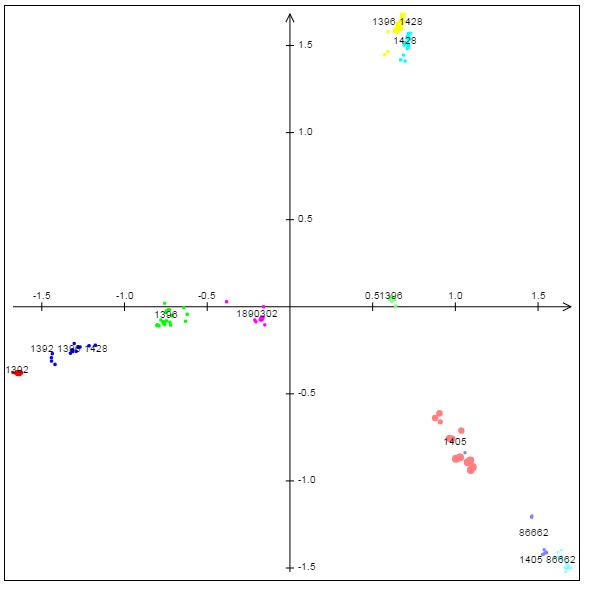
\includegraphics [scale=0.7] {Bacillus_cereus.JPG}


\end{document}


